% This is samplepaper.tex, a sample chapter demonstrating the
% LLNCS macro package for Springer Computer Science proceedings;
% Version 2.20 of 2017/10/04
%
\documentclass[runningheads]{llncs}
%
\usepackage{graphicx}
\graphicspath{ {./img/} }

% Copyright 2017 Sergei Tikhomirov, MIT License
% https://github.com/s-tikhomirov/solidity-latex-highlighting/

\usepackage{listings, xcolor}

\definecolor{verylightgray}{rgb}{.97,.97,.97}

\lstdefinelanguage{Solidity}{
	keywords=[1]{anonymous, assembly, assert, balance, break, call, callcode, case, catch, class, constant, continue, constructor, contract, debugger, default, delegatecall, delete, do, else, emit, event, experimental, export, external, false, finally, for, function, gas, if, implements, import, in, indexed, instanceof, interface, internal, is, length, library, log0, log1, log2, log3, log4, memory, modifier, new, payable, pragma, private, protected, public, pure, push, require, return, returns, revert, selfdestruct, send, solidity, storage, struct, suicide, super, switch, then, this, throw, transfer, true, try, typeof, using, value, view, while, with, addmod, ecrecover, keccak256, mulmod, ripemd160, sha256, sha3}, % generic keywords including crypto operations
	keywordstyle=[1]\color{blue}\bfseries,
	keywords=[2]{address, bool, byte, bytes, bytes1, bytes2, bytes3, bytes4, bytes5, bytes6, bytes7, bytes8, bytes9, bytes10, bytes11, bytes12, bytes13, bytes14, bytes15, bytes16, bytes17, bytes18, bytes19, bytes20, bytes21, bytes22, bytes23, bytes24, bytes25, bytes26, bytes27, bytes28, bytes29, bytes30, bytes31, bytes32, enum, int, int8, int16, int24, int32, int40, int48, int56, int64, int72, int80, int88, int96, int104, int112, int120, int128, int136, int144, int152, int160, int168, int176, int184, int192, int200, int208, int216, int224, int232, int240, int248, int256, mapping, string, uint, uint8, uint16, uint24, uint32, uint40, uint48, uint56, uint64, uint72, uint80, uint88, uint96, uint104, uint112, uint120, uint128, uint136, uint144, uint152, uint160, uint168, uint176, uint184, uint192, uint200, uint208, uint216, uint224, uint232, uint240, uint248, uint256, var, void, ether, finney, szabo, wei, days, hours, minutes, seconds, weeks, years},	% types; money and time units
	keywordstyle=[2]\color{teal}\bfseries,
	keywords=[3]{block, blockhash, coinbase, difficulty, gaslimit, number, timestamp, msg, data, gas, sender, sig, value, now, tx, gasprice, origin},	% environment variables
	keywordstyle=[3]\color{violet}\bfseries,
	identifierstyle=\color{black},
	sensitive=false,
	comment=[l]{//},
	morecomment=[s]{/*}{*/},
	commentstyle=\color{gray}\ttfamily,
	stringstyle=\color{red}\ttfamily,
	morestring=[b]',
	morestring=[b]"
}

\lstset{
	language=Solidity,
	backgroundcolor=\color{verylightgray},
	extendedchars=true,
	basicstyle=\footnotesize\ttfamily,
	showstringspaces=false,
	showspaces=false,
	numbers=left,
	numberstyle=\footnotesize,
	numbersep=9pt,
	tabsize=2,
	breaklines=true,
	showtabs=false,
	captionpos=b
}
	% copy the file from this repo
% Used for displaying a sample figure. If possible, figure files should
% be included in EPS format.
%
% If you use the hyperref package, please uncomment the following line
% to display URLs in blue roman font according to Springer's eBook style:
% \renewcommand\UrlFont{\color{blue}\rmfamily}

\begin{document}
%
\title{Ants-Review: A Protocol For Open Anonymous Peer-Reviews\thanks{}}
%
%\titlerunning{Abbreviated paper title}
% If the paper title is too long for the running head, you can set
% an abbreviated paper title here
%
\author{Bianca Trovò\inst{1,2}\orcidID{0000-0002-6776-2304} \and
Nazzareno Massari\inst{3,4}\orcidID{0000-0002-6638-2174}}
%
\authorrunning{B. Trovò et N. Massari}
% First names are abbreviated in the running head.
% If there are more than two authors, 'et al.' is used.
%
\institute{Sorbonne Université, Faculté des Sciences et Ingénierie, 75005 Paris, France \and
Neurospin research center, CEA/SAC/DSV/I2BM, 91191 Gif-sur-Yvette, France
\email{bianca.trovo@alumni.unitn.it}\\
\and
Alma Mater Politecnico di Torino, 10129 Turin, Italy\and
Independent blockchain engineer, London, UK \\
\email{nazzareno@nazzarenomassari.com}}
%
\maketitle              % typeset the header of the contribution
%
\begin{abstract}
Peer-review is a necessary and essential quality control step for scientific publications. However, the process, which is very costly in terms of time investment, not only is not remunerated but it’s also not recognized by the academic community as a relevant scientific output for a researcher. Therefore, scientific dissemination is affected. Here, to solve this issue we propose a blockchain-based incentive protocol that rewards scientists also for their contributions to other scientists’ work and that builds up a reputational system. We designed a basic Bounty-like contract called AntsReview that allows any author to issue a call for peer-reviewing their scientific publication. If requirements are met, peer-reviews will be audited by an external editor and payed by the Issuer. To promote ethical behaviour the system will implement a quadratic funding on AntsReview.
\keywords{Blockchain  \and Peer-review \and Privacy \and Incentivization.}
\end{abstract}
%
%
\section{Introduction}
blockchain for science here and application to open science and to peer review as a specific case
An increasing body of voices in the scientific community has started to speak up for the need of updating current scientific practices with the advances represented by blockchain technology [2, 8]. As an example, we refer to a ‘manifesto’ written by a few anonymous authors, proposing a blockchain based system of academic endorsement (AES) [1]. Indeed, we could say that in general “specific blockchain characteristics meet the requirements of an open science infrastructure” [3-7]: decentralisation, taking out the need of intermediaries, would make useless depending on highly profiting publishing companies for disseminating scientific work and managing the rules of the peer-review process; immutability of the system in which information can only be appended with tamper proof-time stamping,  but not subsequently modified, would secure the intellectual property and a fairer measure of the scientific contribution of the actors at play during the multiple versions of a paper; transparency (meaning that we have a viewable record of all the transactions), would also make editorial decisions (publish or not publish a study) more transparent and democratic. Finally, cryptographic hashing could allow for a double-blind process that reduces human biases in judgement by assigning hashed pseudonymous to universal researcher identifiers. From all these aspects taken together, a more democratic open peer-review  process could rise, in which merit and power (of access to information, of decision…) is more equally redistributed among the stakeholders (researchers, reviewers, taxpayers).

\section{Background}
\subsection{Peer-review: problem}
Peer-review is the traditional and necessary process at the heart of quality control in science [9, 12], determining the destinies of articles’ publications and therefore of scientific dissemination. However, the current peer-review system is outdated: in the past, it was effective when scholarly communication happened exclusively through printed paper journals, but nowadays, with the high and fast-paced levels of articles productions, its slow and multistage process doesn’t keep up with the times. Indeed, articles submitted to journals can take from months to years after editors’ first scrutiny, going back and forth several review rounds before acceptance for publications. This is mainly due to the fact that the reviewers that are normally appointed by authors and/or editors are actually full-time researchers themselves, who work on a volunteer basis taking time from their primary research. Though things are changing, and now more and more journals encourage a transparent peer review process with the publication of reviewers names and reports, in most of the cases, to guarantee an unbiased output, journals don’t even get credit researchers for this form of unpaid work. On top of this, author-level metrics that measure the scientific impact and productivity of academics, such as the h-index, and are taken into account by the funding agencies, are purely based on the number of citations per each publications while neglecting the full spectrum of scientific contributions (software, data collection, presentations, reviews…). Therefore, peer-reviewing is an intellectual investment without any external return for researchers’ career. A major consequence of not promoting incentives for the quality (and quantity) of peer-reviews is to either have good research unpublished (because unreviewed) and abandoned in preprint archives or bad science published through sloppy and uncritical reviews [5]. Last but not least, the ‘publish or perish’ culture has been more and more inducing malicious behaviour during the peer-review process, such as attempts of scientific fraud (authors trying to review their own papers) and abuse (reviewers producing extremely harsh reviews to damage competitors by blocking the publication of their ideas). Finally, the current peer-review system is usually not double-blind, thus making its decisional process vulnerable to all forms of biases (gender bias, cultural bias, professional bias, etc...). These trust problems are one of the major issues facing scholarly communication.

\subsubsection{Types of peer-review}
\begin{itemize}
    \item single-blind peer review
    \item double-blind peer review
    \item transparent peer review
\end{itemize}

\subsubsection{Traditional peer-review process}
\begin{enumerate}
    \item The author submits a manuscript to the journal.
    \item  An editorial team  assesses the paper for what concerns the requirements of the journal's Author's Guideline (composition, sections...).
    \item An Editor in Chief (EIC) is assigned to the manuscript and checks if the paper meets the scopes of the journal and novelty criteria. If the paper is rejected, it does not go through the consideration process and the editor notifies the author.
    \item If the editorial decision is to send the manuscript for review, the handling editor looks for potential reviewers. Potential reviewers can be suggested by the authors themselves, but usually it's up to the editor to find researchers in the field who are competent enough but not closely related to the study to review.
    \item Candidate reviewers receive the journal's invitation and evaluate acceptance based on their own level of expertise, intrinsic conflicts of interest and time availability. They then accept or decline. If they decline, they might suggest alternative reviewers. Editors keep searching for reviewers until they find two or three reviewers who agree to review the manuscript.
    \item When reviewers engage themselves in delivering peer-review report by a certain deadline, the author(s) are notified. The reviewers identity is usually only know to the editor but is hidden to the authors or the other reviewers themselves. 
    \item Reviewers independently conduct their reviews by exposing in their reports strengths and weaknesses of the manuscript in a point-by-point fashion and submitting a final recommendation to the editor: acceptance, rejection or revision (major or minor).
    \item the handling editor or the editorial team considers all the submitted reports and makes the final decision.
    \item If the decision is a major or minor revision, authors are invited to re-submit a corrected or improved version of the manuscript with a letter to the reviewers. The same reviewers might be contacted again and if they want they can follow up the peer-review process. 
    \item If the decision is a rejection, the editor might indicate another journal where to submit the manuscript. 
    
\end{enumerate}

\subsection{Related work}

Credit for peer review is not a new thing: mostly journals handled it so far with virtual 'badges', certificates of performance, citation in annual editorials but none of these is standardized in a way that has a weight for funders world ranking bodies institutions like imapct factor h-index. 

Crossref primary DOI provider, announced that review reports could be now registered as part of their services
Publons provides a way to keep track of the reviews records and integrate them into academic profiles such as ORCID
ScienceOpen
DEIP
Rubriq provides independent and standardized peer review that can be accepted and shared across all types of journals and distribution systems. Now absorbed by Research Square.
Peerage of Science that provides a journal-independent free service for scientific peer review and publishing. The interesting feature is that it provides also a peer-review of the reviews. 
Blockchain for Peer Review, pilot project sponsored by Digital Science and Katalysis, aims at developing a protocol for storing peer reviews submitted by publishers on a blockchain such that review process can be independently verified and review info is fed to ORCID researcher profiles []

The project will develop a protocol where information about peer review activities (submitted by publishers) are stored on a blockchain. This will allow the review process to be independently validated, and data to be fed to relevant vehicles to ensure recognition and validation for reviewers.  By sharing peer review information, while adhering to laws on privacy, data protection and confidentiality, we will foster innovation and increase interoperability.




\section{System concept}
For the above mentioned reasons, we propose an incentive-based protocol called Ants-Review to reward open peer-reviews while preserving the anonymity of the reviewers. The name originates from the idea that the work behind a finished scientific paper resembles a complex organism such as an anthill, which emerges from the sum of many individualities: in it, all contributions (even if ‘micro’) are essential to the whole and are worth recognition.
This project is intended to be open source and was developed during the ETH Turin 2020 Hackathon and it’s design and attempt of implementation are exposed in the following section.
Anonymity
Accountability
Reputation
Reward
Gamification model 

open identities open reports open participation open interaction open platform ('decoupled review')

\subsection{Design}

\subsubsection{AnstReview process: scenario 1  (journal-dependent)}

\begin{enumerate}
    \item The author submits a manuscript to the journal.
    \item If the papers passes stage 2-3 of editorial decision (appropriateness of style and coherence with the journal's scope)
    \item the editor issues a bounty (\emph{bounty issuance}) for the paper review. Fulfillment rules are set in a smart-contract.
    \item (footnote?) the bounty prize could correspond to part of the article submission fees and article publication fees requested to the authors by the journal.
    \item Reviews fulfilling the smart-contract requirements are validated by the journal editors.
    \item When the reviews are accepted (\emph{bounty fulfillment}), reviewers awarded a token called \emph{ANT}.
    \item Not all reviews will have the same quality and depth. However, each of them might bring up one or more relevant contribution for the sake of improving the manuscript. In order to redistribute the bounty in a fair manner across reviewers, reviews will be voted by the editors with Quadratic Voting.********* POINT OF FAILURE? who votes? 
    
\end{enumerate}

\subsubsection{AnstReview process: scenario 2  (community-driven): 

peer-review is decoupled from journal
or to the pre-print service or to an hypothetical AntsReview platform).
\subsection{Implementation}
AntsReview is a destributed peer-review system which synthetizes successfull ideas from previous systems including The Bounty Network[ref], ERC20[ref], AZTEC Protocol[ref], IPFS[ref], Proof of Existence[ref], ...
\newline The contribution of AntsReview is simply allowing the peer-review process, as a complex system, to emerge as a self-organised ecosystem of authors and peer-reviewers to enhance the complexity of a paper and its validation.
\newline AntsReview represent a new platform to issue peer-reviews and validate scientific papers and a new system for anonymous and open contributions with an incentivization mechanism to reach an ideal state of equilibrium and create value.
\newline The AntsReview Protocol is divided into stack of sub-protocols responsible for different functionality:

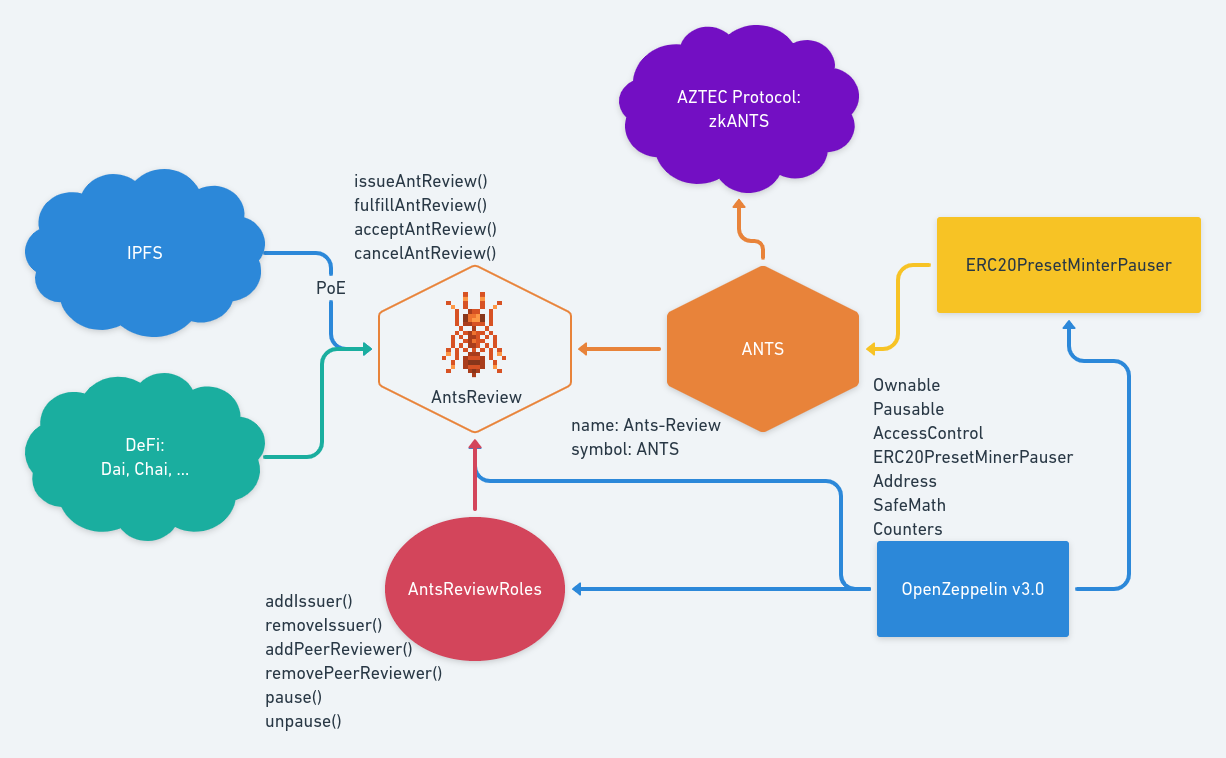
\includegraphics[scale=0.28]{AntsReview}

\begin{enumerate}
  \item \textbf{Bounty} - manage access management and the basic system.
  \item \textbf{Token Economics} - manage system incentivization mechanism integrating ideas from DeFi and Quadratic Funding.
  \item \textbf{Privacy} - mantains the anonymity of the system via AZTEC Protocol.
\end{enumerate}

\subsubsection{Bounty}
AntsReview is the core of the smart contracts deployed on Ethereum Rinkeby's Testnet as shown in the flow-chart[img].
\newline It implements a Bounty-like system where an issuer (author) is asked a serious of actions, to ensure transparency and robustness, regarding the AntReview that he's creating:
\begin{itemize}
  \item to upload the file containing the requirements of the peer-review and the paper into IPFS.
  \item to speficy a deadline in the form of a unix timestamp after wich the fulfillment will no longer be accepted.
  \item to send the amount of ether for the reward.
\end{itemize}

AntsReviewRoles, to ensure integrity of the system, implements an access management, leveraging on AccessControl.sol by OpenZeppelin Library, through the creation of the Roles Issuer and Peer-Reviewer[code].

\begin{lstlisting}[language=Solidity]

pragma solidity 0.6.8;

import "@openzeppelin/contracts/access/AccessControl.sol";

contract AntsReviewRoles is AccessControl {

/// Roles
bytes32 public constant ISSUER_ROLE = keccak256("ISSUER_ROLE");
bytes32 public constant PEER_REVIEWER_ROLE = keccak256("PEER_REVIEWER_ROLE");

}
\end{lstlisting}

In this way, only the Issuer (author) can create a new AntReview.
\newline Once created, an AntReview is available to be fulfilled by Peer-Reviewers, uploading the peer-review on IPFS before the deadline.
\newline The AntReview after being validated is then accepted by the Issuer and paid equally between Peer-Reviewers.
\newline Also, the Issuer can cancel the AntReview at any time and withdraw the amount of ether staked.
\newline One of the key aspects of the protocol is the concept of Proof of Existence, introduced by Stuart Haber & W. Scott Stornetta with the paper "How to time-stamp a digital document".
\newline As the pioneer of blockchain an cited by Bitcoin whitepaper, they were in a mission to solve the problem of immutability of digital records that became reality with the Blockchain and Bitcoin as its first application.
\newline In Ethereum the concept of immutablity is achieved via the blockchain and proof of work consesus algorithm by a chain of timestamped block hashes that are secured by miners competing computations.
\newline AntsReview is evaluating the advantages of storing the hashes of the peer-reviews into a Merkle Tree to achieve immutability.












\subsubsection{Token Economics}

\subsubsection{Quadratic Funding}

\subsubsection{Privacy}

\subsubsection{DAO}


\subsubsection{Future steps}
Future integrations that were not contemplated in the above presented PoC /demo but that we plan to cover for the development of the AntsReview bounty include: an ERC20 token, named Ant,  symbol ANT; Proof of Existence (PoE) service; memory storage on IPFS; moreover, since we wanted to anonymize peer-reviews to protect the contributors privacy, we would like to implement on the ANT token a fast, non-interactive type of zero-knowledge privacy protocol to enable private transactions on Ethereum. Zero-knowledge proof is a mathematical cryptographic method that through values permutations allows one party (the prover) to prove to another (the verifier) the veracity of a statement, without having to reveal what the statement is. We will use ZK-SNARKs (which stands for “Zero-Knowledge Succinct Non-Interactive Argument of Knowledge”) via the open source libraries of AZTEC protocol [15]. We will also use Ethereum Name Service (ENS) [14] to allow for human-readable Ethereum addresses; Upgradability Design Patterns [13] via Proxy, to allow the logic to be extended and improved; De-Fi integrations such as Dai, Chai. Finally, we would like to propose for AntsReview Quadratic Funding, a design written by Vitalik Buterin and co [20] and which applies concepts inspired by quadratic voting to funding public goods.

\section{Discussions}

- a change is already happening: specially new born publishers are opening up review process (BioMed Central, ELife, Frontiers, PeerJ, F1000 Research) -- from 2020 also Nature declaired that will do the same. 

- new business model? at some point pre-print platforms (dissemination) might want to integrate peer-review (validation) into their platforms - dissociation of initial scientific dissemination and scientific validation will force publishing industry to adapt: how will they justify their added value? as Tennant points out: branding archiving 

- peer reviews requires a standard: building smart-contracts for peer-reviews might set a first step in this direction 

- community-organized peer  reviews: peer reviews will be more and more out of the hands of publishers, researchers will be the ones seeking the papers to review (like in Rubriq). 

future of quality control and moderation: open participation model, community-driven | certification and reputation: expansion of reviewer pool with fewer barriers to enter and more inclusion of young scientists, reputation build within community and not journals 

- portable peer review not only within a consortium of journals 

-value of peer review as 'academic capital' recognized by research funders and hiring committees

-a bit off topic but: automated peer review (services such as StatReviewers) might fasten the formal aspects of the job allowing reviewers to focus on the content.

\section{Conclusion}
In this paper we addressed a central problem within the quality control academic dissemination: the peer-review process. We showed how blockchain technology could provide an efficient and viable solution and open up possibile directions for a change in paradigm in scientific communication. We proposed an incentive mechanism that could solve the problems of lack of acknowledgment and trust during peer-review. We exposed the architecture of our project and our Proof of Concept (PoC) for which we adopted cutting-edge tools from the open source blockchain community.

\subsubsection{Supplementary material}
Our open source code is available at the Github repository. A demo of the project is available at Youtube channel.

\subsubsection{CRediT Authorship Contribution Statement}
TDB

\subsubsection{Declaration of Competing Interest}
The authors declare no competing interests.

\subsubsection{Acknowledgements} We would like to thank Matteo A. Tambussi for his comments and edits.

% ---- Bibliography ----
%
% BibTeX users should specify bibliography style 'splncs04'.
% References will then be sorted and formatted in the correct style.
%
\bibliographystyle{splncs04}
\bibliography{references.bib}

\end{document}
